\documentclass{article}
\usepackage{geometry}
 \geometry{
 a4paper,
 total={170mm,270mm},
 left=20mm,
 top=10mm,
 }
\usepackage{graphicx}
\usepackage{listings}
\usepackage{float}
\usepackage{enumitem}
\usepackage{caption}
\usepackage{amsmath}
\usepackage{datetime}
\usepackage{multirow}
\newcommand*{\addheight}[2][.5ex]{%
  \raisebox{0pt}[\dimexpr\height+(#1)\relax]{#2}%
}
\newdate{date}{23}{09}{2016}
\date{\displaydate{date}}
\title{\textbf{Machine Learning - CSCI 5622} \\
HW 3 - SVM}
\author{\textbf{Santhanakrishnan Ramani}}
\begin{document}
\maketitle

\section*{Analysis}
\begin{enumerate}
\item
Sklearn implementation of support vector machines to train a classifier to distinguish 3's from 8's,
\begin{lstlisting}
sv.fit(data.x_train,data.y_train)
\end{lstlisting}

The Accuracy is \textbf{0.969}\\
The Confusion Matrix is 
\begin{minipage}[b]{0.4\textwidth}
    \begin{tabular}{l r|l l}                      
		& \multicolumn{1}{r|}{} &3   &8   \\ \cline{2-4}
		& \multicolumn{1}{r|}{3} &996   &34  \\
		& \multicolumn{1}{r|}{8} &29   &280  \\ 
	\end{tabular}
\end{minipage} 

\item
Performance of SVM for various values of C using linear, rbf kernels

\begin{table}[h!]
    \begin{minipage}{.5\textwidth}
    \centering
	\begin{tabular}{|l|l|l|}
	\hline
	C & Kernel & Accuracy\\
	\hline
	0.01 & linear & 0.968612064738 \\
	0.1  & linear & 0.97106424718  \\
	1    & linear & 0.968121628249 \\
	2    & linear & 0.966159882295 \\
	5    & linear & 0.96468857283  \\
	10   & linear & 0.963707699853 \\
	100  & linear & 0.95831289848 \\
	\hline
	\end{tabular}
	\end{minipage}
    \begin{minipage}{.5\textwidth}
    \centering
	\begin{tabular}{|l|l|l|}
	\hline
	C & Kernel & Accuracy\\
	\hline
	0.01 & rbf & 0.917606669936 \\
	0.1  & rbf & 0.954389406572 \\
	1    & rbf & 0.969102501226 \\
	2    & rbf & 0.972535556645 \\
	5    & rbf & 0.978911230996 \\
	10   & rbf & 0.981363413438 \\
	100  & rbf & 0.989700833742 \\
	\hline
	\end{tabular}
	\end{minipage}
\end{table}

From the above table, we can see that when using linear kernel, which is similar to a  svm without the kernel trick, as you increase the value of C above 0.1 you start penalizing more for misclassification and try to fit more data to its correct class, so when the data isn't linearly separable the accuracy decreases. In case of rbf kernel, as the data is projected to a higher dimension, the data may become more separable and as you increase the value C you try to predict more values correctly and accuracy increases.

\item
Examples of support vectors from each class when using a linear kernel.
\begin{table}[H]
\centering
\begin{tabular}{|c|c|c|c|}
	\hline
	\addheight{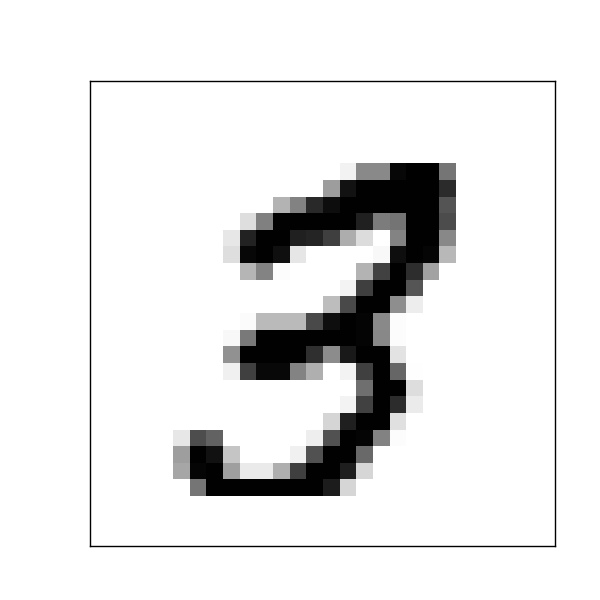
\includegraphics[width=40mm]{images/3a.png}} &
	\addheight{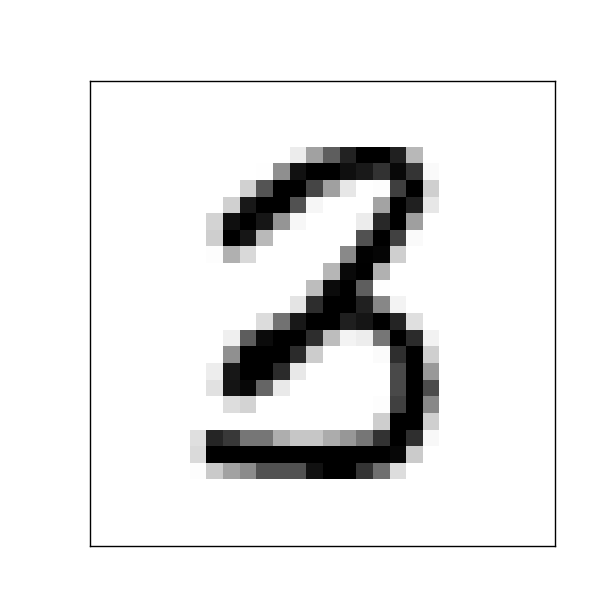
\includegraphics[width=40mm]{images/3b.png}} &  
    \addheight{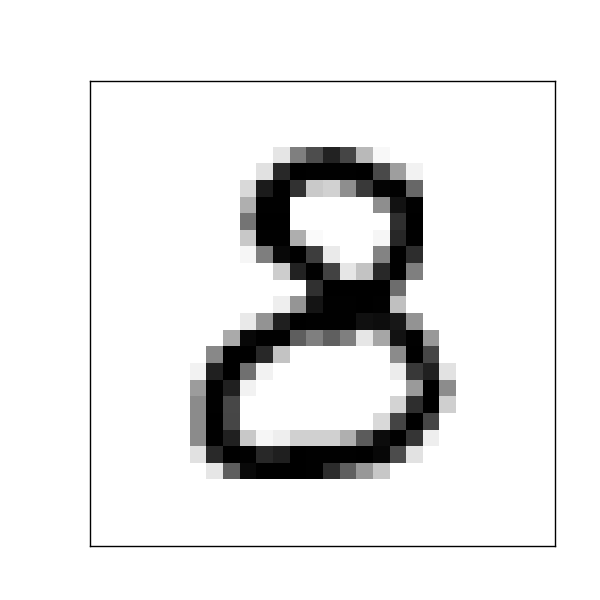
\includegraphics[width=40mm]{images/8a.png}} &
    \addheight{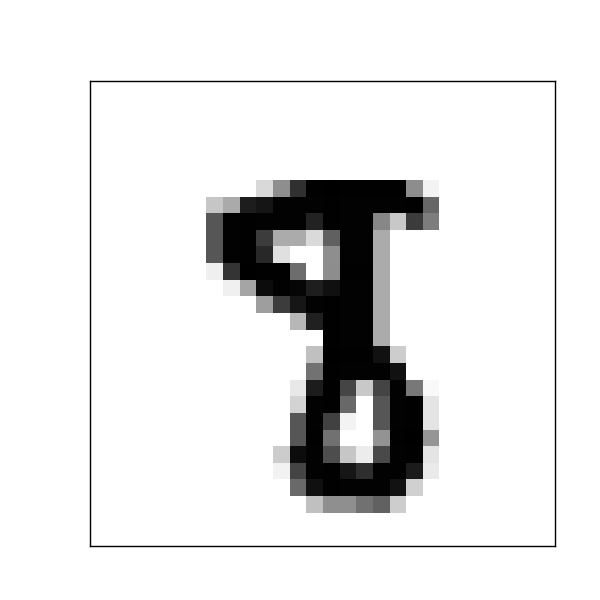
\includegraphics[width=40mm]{images/8b.png}} \\
    \hline 
\end{tabular}
\end{table}
\end{enumerate}

\end{document}
	